\documentclass{article}

\usepackage{graphicx}
\usepackage{tikz}
\usepackage{tikzsymbols}
\usetikzlibrary{calc,patterns,shapes.geometric}
\pagestyle{empty}
\usepackage[margin=0pt]{geometry}
\geometry{papersize={14in,12in}}

\def\centerarc[#1](#2)(#3:#4:#5){\draw[#1] ($(#2)+({#5*cos(#3)},{#5*sin(#3)})$) arc (#3:#4:#5);}

\begin{document}
	\begin{figure}
		\centering
		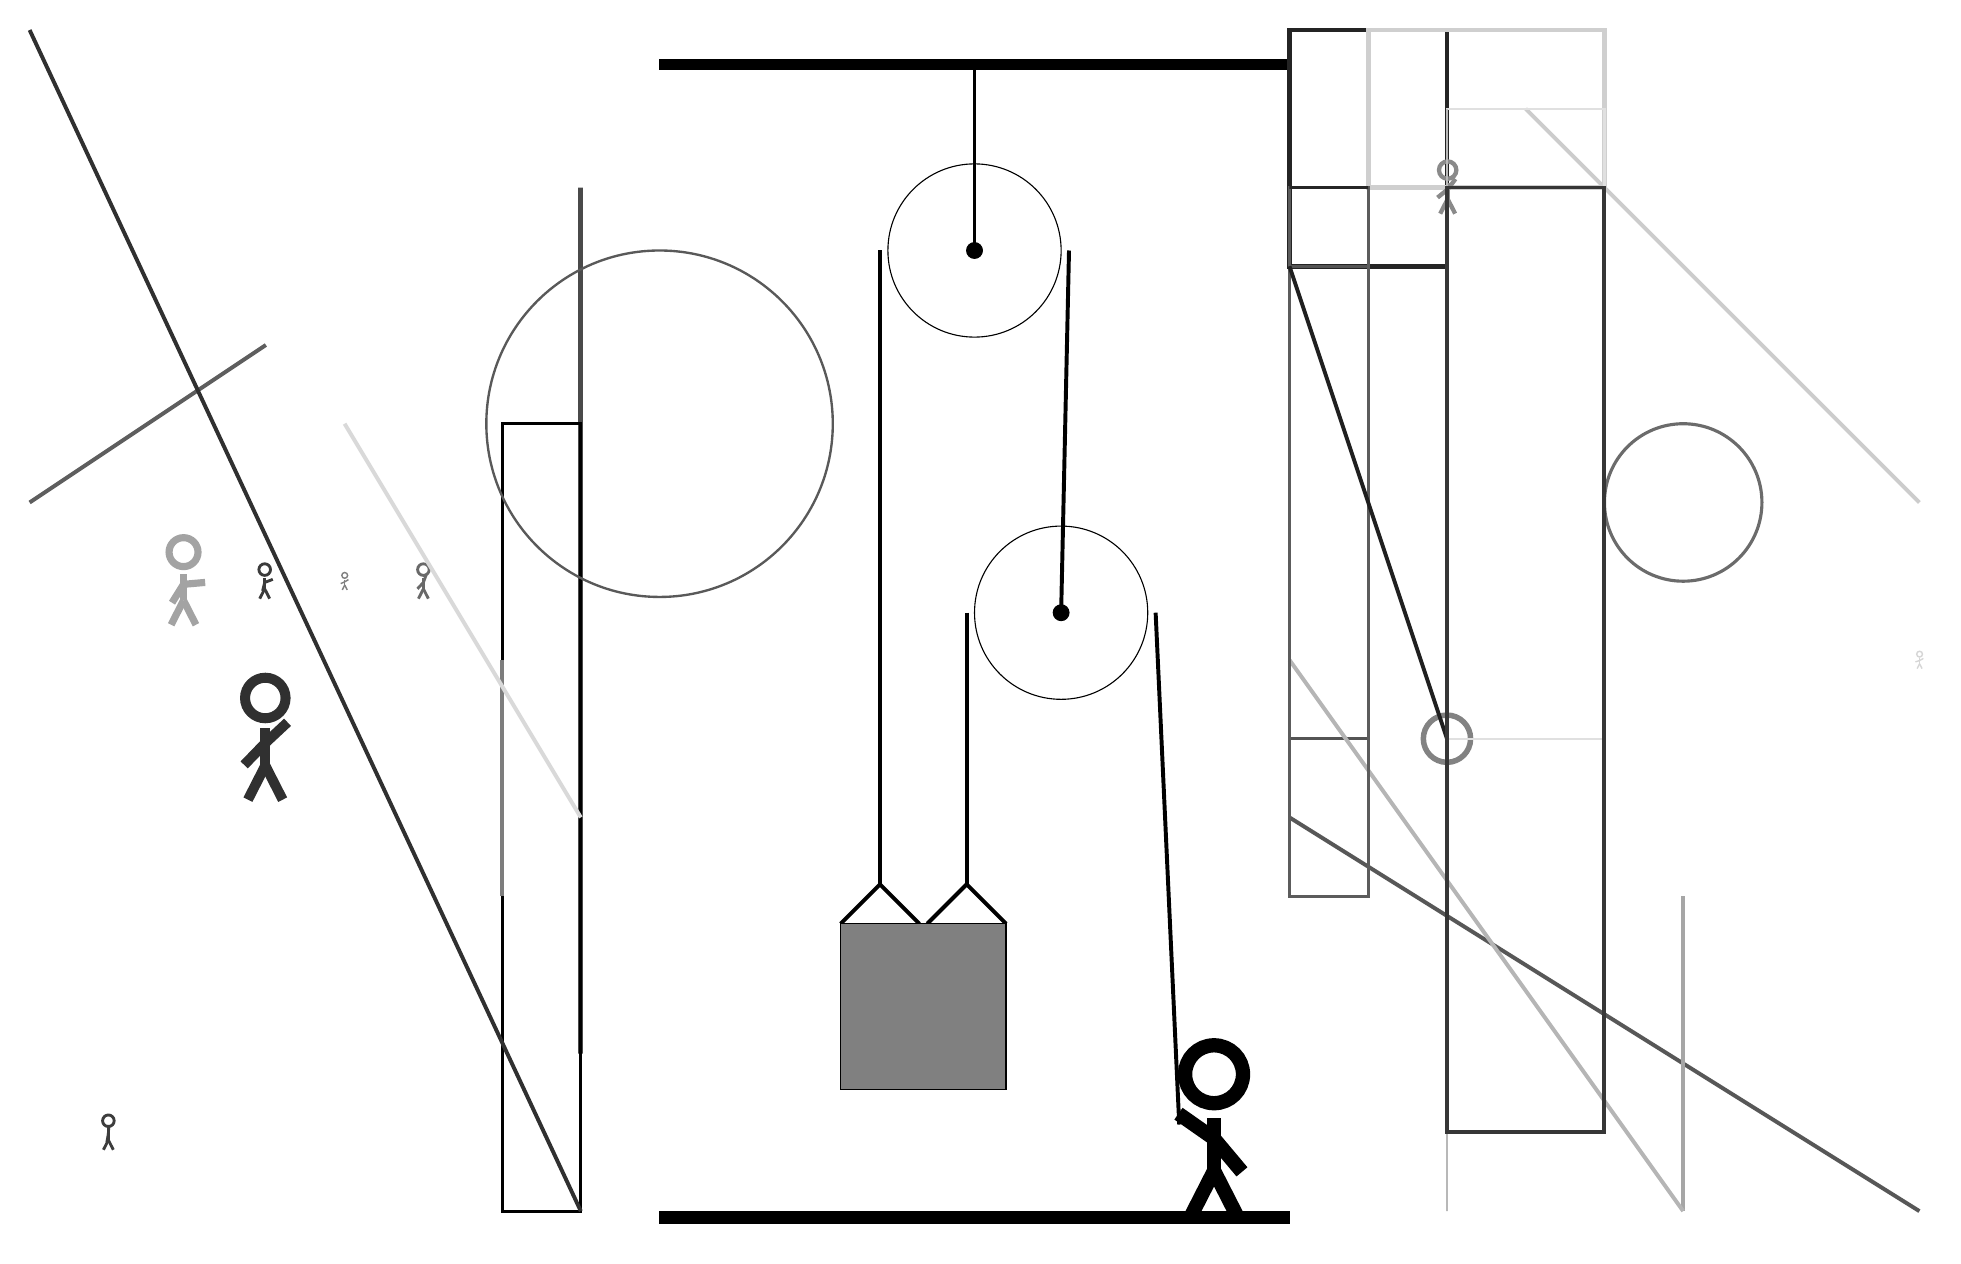
\begin{tikzpicture}
			%%%%% START %%%%%
			
			\draw[fill=black] (-2, 11.5) rectangle (6, 11.625);
			
			\draw (2, 9.2) circle (1.1);
			\draw[fill=black] (2, 9.2) circle (0.1);
			\draw[thick] (2, 9.2) -- (2, 11.5);
			
			\draw (3.1, 4.6) circle (1.1);
			\draw[fill=black] (3.1, 4.6) circle (0.1);
			
			\draw[line width = 0.5mm]  (0.3, 0.65) -- (0.8, 1.15) -- (1.3, 0.65);
			\draw[line width = 0.5mm]  (1.4, 0.65) -- (1.9, 1.15) -- (2.4, 0.65);
			\draw[fill=black!50] (0.3, 0.65) rectangle (2.4, -1.45);
			
			\draw[line width = 0.5mm] (0.8, 9.2) -- (0.8, 1.15);
			\centerarc[line width = 0.5mm](2, 9.2)(0:180:1.2000000000000002);
			\draw[line width = 0.5mm] (3.2, 9.2) -- (3.1, 4.6);
			\draw[line width = 0.5mm] (1.9, 4.6) -- (1.9, 1.15);
			\centerarc[line width = 0.5mm](3.1, 4.6)(0:180:1.2000000000000002);
			\draw[line width = 0.5mm] (4.3, 4.6) -- (4.6, -1.9);
			
			\node[line width=0.5mm, color=black!59] at (-5, 5) {\Strichmaxerl[2][47][70]};
			
			\draw[line width=0.5mm, color=black!66](6, 2) -- (14, -3);
			\draw [line width=0.7mm, color=black!49](8, 3) circle (0.3);
			\draw[line width=0.6mm, color=black!86] (6, 12) rectangle (8, 9);
			\draw[line width=0.5mm, color=black!20](9, 11) -- (14, 6);
			\draw[line width=0.5mm, color=black!79](10, 12) -- (10, -1);
			
			\draw[line width=0.4mm, color=black!56] (8, 5) rectangle (8, 6);
			
			\draw[line width=0.6mm, color=black!71] (-3, 10) rectangle (-3, -1);
			\draw[line width=0.5mm, color=black!63](-7, 8) -- (-10, 6);
			\draw[line width=0.4mm, color=black!67] (6, 3) rectangle (7, 9);
			
			\draw[line width=0.5mm, color=black!35](11, -3) -- (11, 1);
			
			\draw[line width=0.5mm, color=black!29](11, -3) -- (6, 4);
			\draw[line width=0.4mm, color=black!100] (-4, -3) rectangle (-3, 7);
			
			\draw [line width=0.4mm, color=black!58](11, 6) circle (1.0);
			\node[line width=0.3mm, color=black!36] at (-8, 5) {\Strichmaxerl[5][58][5]};
			\draw[line width=0.6mm, color=black!19] (7, 10) rectangle (10, 12);
			
			\node[line width=0.4mm, color=black!81] at (-7, 3) {\Strichmaxerl[7][46][43]};
			\draw[line width=0.4mm, color=black!64] (6, 10) rectangle (7, 1);
			\node[line width=0.6mm, color=black!76] at (-9, -2) {\Strichmaxerl[2][80][87]};
			\node[line width=0.7mm, color=black!46] at (8, 10) {\Strichmaxerl[3][39][53]};
			\draw[line width=0.5mm, color=black!81](-3, -3) -- (-10, 12);
			
			\draw[line width=0.5mm, color=black!51](-4, 4) -- (-4, 1);
			
			\draw [line width=0.3mm, color=black!65](-2, 7) circle (2.2);
			\draw[line width=0.5mm, color=black!88](8, 3) -- (6, 9);
			\draw[line width=0.5mm, color=black!15](-3, 2) -- (-6, 7);
			
			\draw[line width=0.3mm, color=black!85] (7, 10) rectangle (6, 10);
			\draw[line width=0.3mm, color=black!12] (8, 11) rectangle (10, 3);
			\draw[line width=0.2mm, color=black!28] (8, -3) rectangle (8, 11);
			
			\node[line width=0.5mm, color=black!50] at (-6, 5) {\Strichmaxerl[1][24][31]};
			\node[line width=0.5mm, color=black!16] at (14, 4) {\Strichmaxerl[1][17][29]};
			\node[line width=0.4mm, color=black!77] at (-7, 5) {\Strichmaxerl[2][76][21]};
			
			\draw[line width=0.5mm, color=black!79] (8, 10) rectangle (10, -2);
			
			\node at (5, -2) {\Strichmaxerl[10][-35][-50]};
			
			\draw[fill=black] (-2, -3) rectangle (6, -3.15);
			
			%%%%% END %%%%%
		\end{tikzpicture}
	\end{figure}	
\end{document}